\section{Early Exit Neural Networks}

Early Exit Neural Networks (EENNs) are designed to provide predictions within a fixed, often reduced, inference time. 
These networks allow predictions to be made at intermediate layers, reducing the computational load and energy consumption when full-depth inference is unnecessary. 
However, this improvement in computational efficiency comes at the cost of increased memory usage, due to the added classifier layers required at various depths of the network.

Deep Neural Networks (DNNs) are widely used across diverse domains such as image classification, object recognition, and predictive analytics. 
Traditionally, DNNs are structured as sequential stacks of layers, with predictions generated only after all layers have been processed. 
While this ensures maximal feature extraction, it introduces several limitations: high computational demand, fixed and potentially long inference time, and risk of overfitting and other inefficiencies.

EENNs address these issues by incrementally processing inputs and making early predictions once sufficient confidence is achieved. 
This is enabled by Early Exit Classifiers (EECs) which are auxiliary classifiers inserted at intermediate stages of the network. 
The original model, without these exits, is referred to as the Backbone Network.
EENNs leverage the observation that:
\begin{itemize}
    \item Many input samples can be accurately classified with shallow sub-networks.
    \item The Lottery Ticket Hypothesis suggests that smaller, well-initialized sub-networks can match the performance of deeper ones.
    \item Overthinking can degrade performance, where deeper layers can override correct early predictions.
\end{itemize}
\noindent By allowing some inputs to exit early, EENNs not only reduce inference time but may also improve accuracy in certain scenarios.

\paragraph*{Properties}
EENNs bring several advantages:
\begin{itemize}
    \item \textit{Reduced inference time}: early exits prevent unnecessary computation for easy-to-classify inputs.
    \item \textit{Decreased overfitting}: simpler models reduce the risk of overfitting.
    \item \textit{Mitigation of vanishing gradients and overthinking}: earlier exits alleviate issues typically associated with deep architectures.
    \item \textit{Flexible deployment}: EENNs can be distributed across multi-tier architectures.
    \item \textit{Dynamic trade-off}: users can adjust thresholds to balance accuracy and latency at runtime.
    \item \textit{Improved interpretability}.
\end{itemize}
\noindent Notably, earlier classifiers are not necessarily less accurate than deeper one.

\subsection{Architecture}
\paragraph*{Classifier}
Let $f_i(x)$ denote the output of an intermediate layer $i$ in the backbone network.
An EEC is added at that point to produce a prediction:
\[\bar{y}_i=C_i(f_i(x))\]
Thus, the EENNs yields a sequence of predictions $\bar{y}_1,\bar{y}_2,\dots,\bar{y}_N$, in addition to the final output $\hat{y}$.
These predictions may vary in accuracy depending on the layer at which they are computed.
\begin{figure}[H]
    \centering
    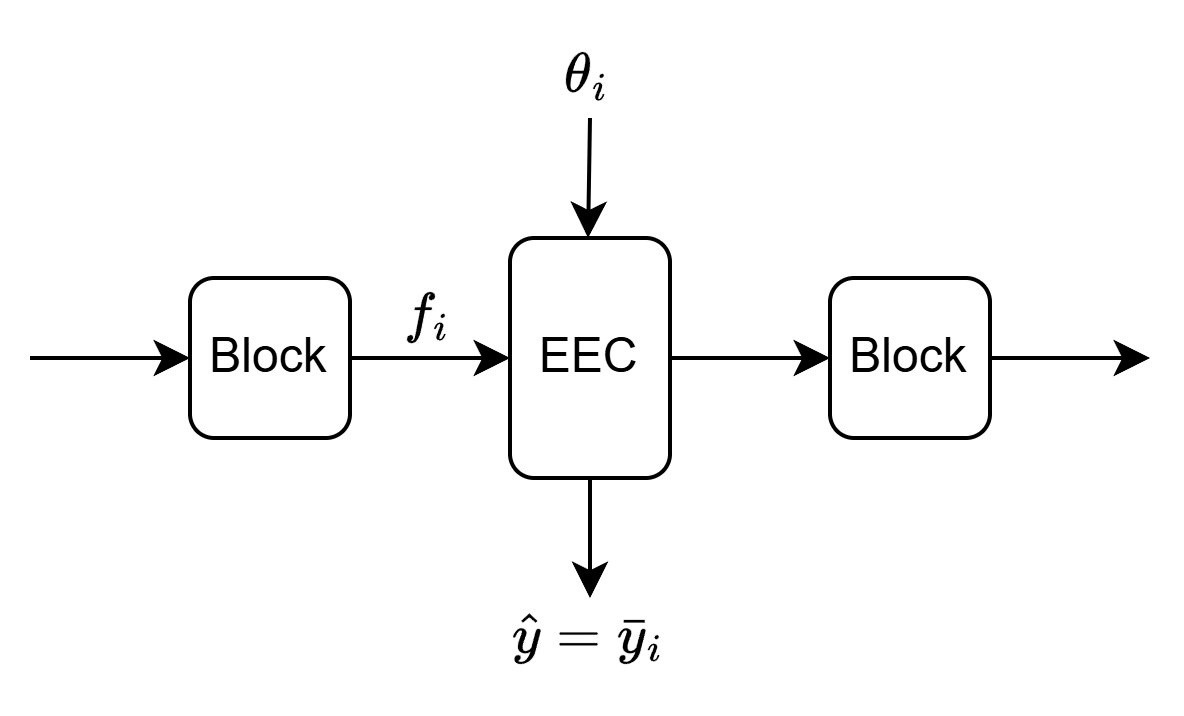
\includegraphics[width=0.75\linewidth]{images/eeai11.png}
    \caption{Early Exit Classifier}
\end{figure}

\paragraph*{Selection scheme}
To determine whether an input should exit early, each EEC is associated with a decision function governed by a threshold.
The decision function $D_i(x)$ compares the confidence score $C_i (x)$  against a predefined threshold $\theta_i$: 
\[D_i(x) = C_i (x) \geq \theta_i\]
\noindent If the confidence score exceeds the threshold, the model halts further processing and outputs $\bar{y}_i$ as the final prediction.
Otherwise, the input continues to propagate through the network.

Here, $N$ is the total number of EECs. 
These thresholds $\theta_i$ are key hyperparameters that control the trade-off between inference time and classification accuracy.
\begin{figure}[H]
    \centering
    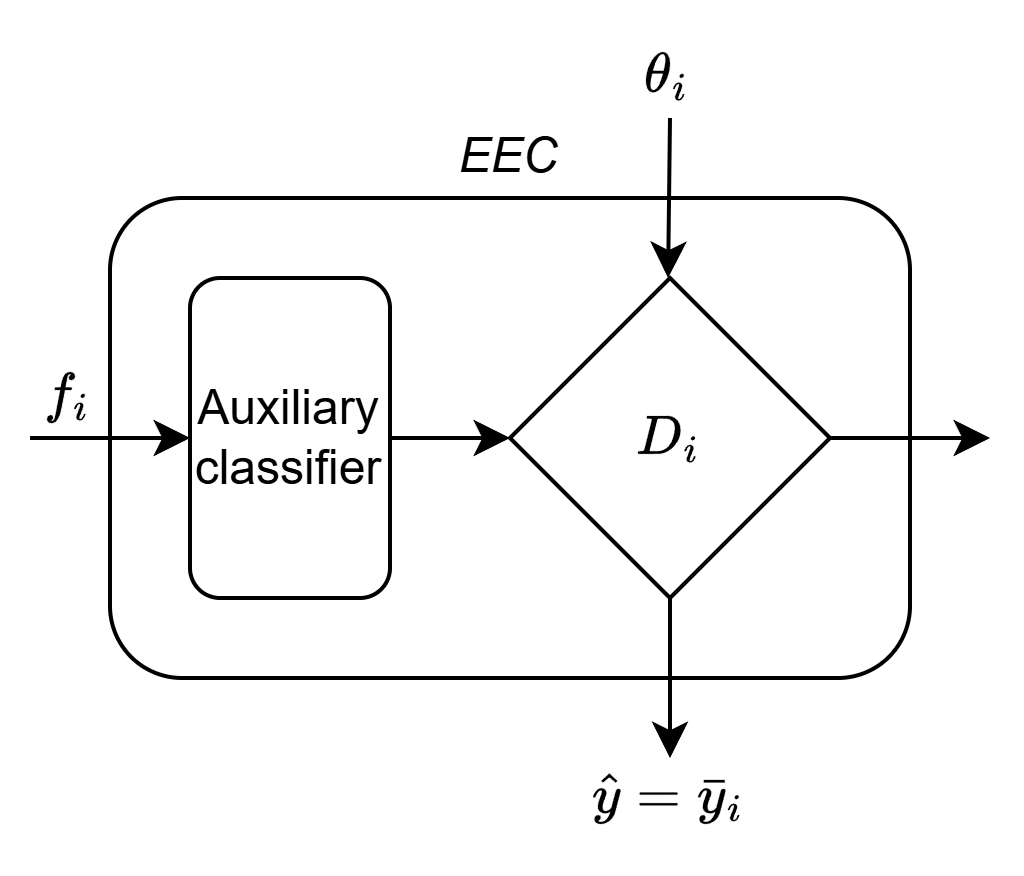
\includegraphics[width=0.75\linewidth]{images/eeai12.png}
    \caption{Early Exit Auxiliary Classifier and Decision Function}
\end{figure}